\item \textbf{{[}JJC/PRELIM/9597/2018/P2/Q1{]} }

J \& J Dental Care has a team of freelance dentists. As there are
two dental treatment rooms in the clinic, only two dentists may be
on duty each day. The clinic manager finalises the monthly duty roster
a week before the new month commences. Every patient has to either
call or visit the clinic to book an appointment. The receptionist
handling the booking will require the following details: 
\begin{itemize}
\item patient name 
\item postal code 
\item dentist requested (optional)
\item date requested 
\end{itemize}
The receptionist checks the hard copy files to ensure that the patient
is registered with the clinic and views the availability in the appointments
book. After the dentist, date and time have been finalised, the patient\textquoteright s
appointment will be recorded in the appointments book.

At the beginning of each day, the receptionist types an appointment
list for each of the dentists working that day. The list contains
patients\textquoteright{} names and their respective timings. 

When patients arrive at the clinic for their appointments, they announce
their names to the receptionist and the receptionist will enter the
treatment rooms to inform the dentists. 

The clinic has decided to replace this manual system with a computerised
system. 

A system developer is employed to carry out the project. The first
task assigned to the system developer is to write a project proposal.
\begin{enumerate}
\item One section of the project proposal is the Problem Statement which
lists the problems in the current system. Write the Problem Statement.
\hfill{}{[}4{]}
\item Explain why the problem must be defined accurately. \hfill{}{[}2{]}
\item Describe and justify three methods which can be used to determine
the requirements for the computerised system.\hfill{} {[}6{]}
\item As a result of the analysis carried out, a diagram is used to show
entities and data flow of the \uline{appointment booking process
only}. Draw a suitable diagram.\hfill{} {[}6{]}
\end{enumerate}
The system developer has drawn up an initial plan of the work involved: 
\noindent \begin{center}
\begin{tabular}{|c|l|c|}
\hline 
\textbf{Stage} & \textbf{Activity} & \textbf{Weeks}\tabularnewline
\hline 
A & Produce design & 5\tabularnewline
\hline 
B & Identify requirements & 3\tabularnewline
\hline 
C & Implement code & 9\tabularnewline
\hline 
D & Perform black box testing & 2\tabularnewline
\hline 
E & Perform acceptance testing & 3\tabularnewline
\hline 
F & Prepare documentation & 6\tabularnewline
\hline 
\end{tabular} 
\par\end{center}

From the work breakdown, a Program Evaluation Review Technique (PERT)
chart is constructed. 
\begin{center}
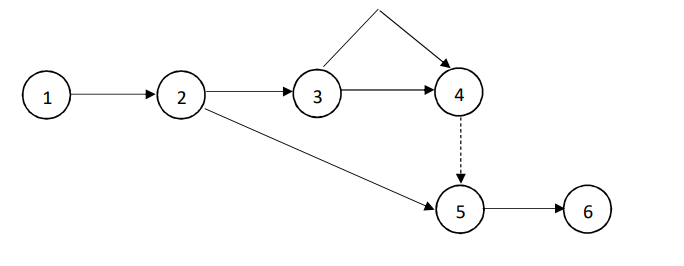
\includegraphics[width=0.5\paperwidth]{C:/Users/Admin/Desktop/Github/question_bank/LyX/static/img/9597-JJC-2018-P2-Q1-1}
\par\end{center}
\begin{enumerate}
\item[(e)]  Complete the PERT chart by adding the stages and their respective
durations in the correct sequence.\hfill{} {[}4{]}
\item[(f)]  State the critical path.\hfill{} {[}1{]}
\item[(g)]  State the minimum time in which the project could be completed.\hfill{}
{[}1{]}
\item[(h)]  The first activity commences at Week 0. For activity D: 
\begin{itemize}
\item state the earliest start time. 
\item state the latest finish time.\hfill{}{[}2{]}
\end{itemize}
\item[(i)]  Two stages start and end at the same nodes. 
\begin{itemize}
\item Re-draw the PERT chart by using an additional dummy stage separating
them. 
\item Explain the purpose of the dummy stage. \hfill{} {[}2{]}
\end{itemize}
\item[(j)]  List two types of documentation produced for this project. \hfill{}{[}2{]}
\end{enumerate}
The computerised system will use a database. In the updated system
the dentists will be given a hand-held device, that is networked,
to use in their rooms for accessing the patient records. 
\begin{enumerate}
\item[(k)]  Describe two other uses for the hand-held device. \hfill{} {[}2{]}
\item[(l)]  Describe a possible ethical concern raised by this new system. \hfill{}{[}2{]}
\item[(m)] An alternative solution for this project is to use cloud computing.
Describe how each of the three types of cloud computing services may
be used for the new project. \hfill{} {[}6{]}
\end{enumerate}